\section{Interpretations are useful: Penalizing Explanations to Align Neural Networks with Prior Knowledge}
In their paper \textit{Interpretations are useful: Penalizing Explanations to Align Neural Networks with Prior Knowledge}\cite{interps-are-useful},
Rieger, Singh, Murdoch and Yu propose a method to penalize a model during training,
if it does not align with the prior knowledge of the dataset (for instance that a ruler shouldn't be used to classify a benign tumor).
To show examples of their method, they (among other things) train a model on the ISIC dataset \cite{ISIC_Dataset_2018}.

Here, they are able to use saliency maps (see section \ref{sec:saliency_maps}) to see, that the model is using rulers to classify benign lesions.
In Figure \ref{fig:interps-are-useful-saliency-maps}, their figure has been shown that clearly indicates that the model is using the rulers.
From these saliency maps, they conclude that the model is using the rulers to classify malignant lesions.
\begin{figure}[h]
    \centering
    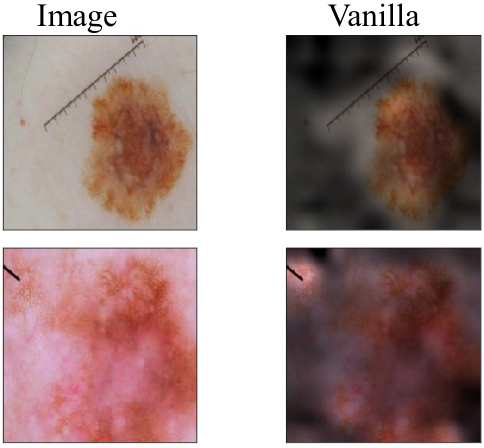
\includegraphics[width=0.6\textwidth]{./images/interps-are-useful-saliency-maps.png}
    \caption{Cutout of Figure S6 from \cite{interps-are-useful}. Original description: \textit{
        Both networks learnt that proportionally more images with malignant lesions feature a ruler next to the lesion. To make
        comparison easier, we visualize the heatmap by multiplying it with the image. Visible regions are important for classification
    }}
    \label{fig:interps-are-useful-saliency-maps}
\end{figure}